% ---
% 01. Cinco casas de Manoel Amoedo y Amoedo na rua das Pitangueiras
% ---

\afterpage{
\begin{a3paisagem}
\begin{figure}[!h]
\centering
\caption{Projecto de construção para cinco casas na Rua 25 de Março, freguezia de Brotas (1892). }
\includegraphics[width=1\textwidth]{8-anexos/plantas/01-1distrito/04-agripino-dorea/agripinodorea-manoelamoedoyamoedo-1892.jpg}{\footnotesize \par \textbf{Fonte:} \textbf{BR BAAHMS}, Fundo ``Intendência'', Série ``Processos de Licenciamento de Reforma e Ampliação de Edificações'', Subsérie ``Requerimentos e Plantas -- Brotas'', caixa 04. \par Projeto de José Celestino dos Santos. O mais antigo entre todos os projetos pesquisados é exatamente o de construção de pequenas casas para alugar na rua das Pitangueiras, de propriedade do comerciante espanhol Manoel Amoedo y Amoedo. }
\label{fig:manoelamoedoyamoedo}
\end{figure}
\end{a3paisagem}
}

% ---
% 02. Seis casas de Antonio Ribeiro da Cunha na rua da Alegria do Castro Neves
% ---

\afterpage{
\begin{a3paisagem}
\begin{figure}[!h]
\centering
\caption{Projecto para a construção de seis pequenas casas que o Snr. Antonio Ribeiro da Cunha pretende fazer na rua da Alegria districto de Brotas (1897). }
\includegraphics[width=1\textwidth]{8-anexos/plantas/01-1distrito/10-alegria/alegriadocastroneves-antonioribeirodacunha-seiscasas.jpg}{\footnotesize \par \textbf{Fonte:} \textbf{BR BAAHMS}, Fundo ``Intendência'', Série ``Processos de Licenciamento de Reforma e Ampliação de Edificações'', Subsérie ``Requerimentos e Plantas -- Brotas'', caixa 10. \par Projeto de autor desconhecido. Casas geminadas bem à moda das ``casas para operários'' que lhe sucederam: pequenas, desadornadas, e sobretudo baratas. }
\label{fig:antonioribeirodacunha}
\end{figure}
\end{a3paisagem}
}

% ---
% 03. Casa rural de Francisco Ventura na rua do Sangradouro
% ---

\afterpage{
\begin{a3paisagem}
\begin{figure}[!h]
\centering
\caption{Projecto de casa para o sr. Francisco Ventura (1901). }
\includegraphics[height=0.9\textheight]{8-anexos/plantas/01-1distrito/15-sangradouro/sangradouro-franciscoventura-casa01.jpg}{\footnotesize \par \textbf{Fonte:} \textbf{BR BAAHMS}, Fundo ``Intendência'', Série ``Processos de Licenciamento de Reforma e Ampliação de Edificações'', Subsérie ``Requerimentos e Plantas -- Brotas'', caixa 15. \par Projeto de Manoel R. F. Muniz. Hoje não mais existente, a construção é uma das típicas casas rurais do Sangradouro, um dos limites da urbanização no antigo 1º Distrito na alvorada da Primeira República. }
\label{fig:franciscoventura}
\end{figure}
\end{a3paisagem}
}

% ---
% 04. Casa mista de negócios do capitão Valentin Duran Suarez na rua das Pitangueiras
% ---

\afterpage{
\begin{a3paisagem}
\begin{figure}[!h]
\centering
\caption{Projecto para a construção de uma casa na rua do Dr. Agrippino Dorea nº 22, districto de Brotas, pertencente ao Ilmo. Snr. Capitão Valentin Duran Suarez (1908). }
\includegraphics[height=0.9\textheight]{8-anexos/plantas/01-1distrito/04-agripino-dorea/agripinodorea-valentinduransuarez.jpg}{\footnotesize \par \textbf{Fonte:} \textbf{BR BAAHMS}, Fundo ``Intendência'', Série ``Processos de Licenciamento de Reforma e Ampliação de Edificações'', Subsérie ``Requerimentos e Plantas -- Brotas'', caixa 040. \par Projeto de Antonio Leite da Luz. Este projeto destacou-se entre todos por ser o único no distrito inteiro a combinar uso residencial e comercial no mesmo imóvel: o térreo abre-se com uma ``Area para negocio'' e  ``Bilhar'', separados por um corredor das duas salas, dispensa, cozinha e banheiro existentes no térrero, havendo ainda mais duas salas, cinco quartos, uma alcova e uma capela no ``pavimento nobre''. }
\label{fig:valentinduransuarez}
\end{figure}
\end{a3paisagem}
}

% ---
% 05. Casa rural de Ricardo da Silva Teixeira Machado na rua do Sangradouro
% ---

\afterpage{
\begin{a3paisagem}
\begin{figure}[!h]
\centering
\caption{Projecto para construcção de um andar da casa na roça ao Sangradouro, dist. de Brotas, pertencente ao Snr. Ricardo da Silva Teixeira Machado (1915). }
\includegraphics[height=0.9\textheight]{8-anexos/plantas/01-1distrito/15-sangradouro/sangradouro-ricardodasilvateixeiramachado-constroiandarnacasas.jpg}{\footnotesize \par \textbf{Fonte:} \textbf{BR BAAHMS}, Fundo ``Intendência'', Série ``Processos de Licenciamento de Reforma e Ampliação de Edificações'', Subsérie ``Requerimentos e Plantas -- Brotas'', caixa 15. \par Projeto de Arthur Santos. Ainda era possível falar de ``roças'' no Sangradouro em 1915, evidenciando até onde avançara a urbanização no antigo 1º Distrito. }
\label{fig:ricardodasilvateixeiramachado}
\end{figure}
\end{a3paisagem}
}

% ---
% 06. Vinte casas de José Antonio Ramos na rua do Castro Neves
% ---

\afterpage{
\begin{a3paisagem}
\begin{figure}[!h]
\centering
\caption{Projecto para a construção de 20 casas, para operarios, ao Castro Neves, districto de Brotas, que pretende fazer o snr. José Antonio Ramos (1919). }
\includegraphics[height=0.9\textheight]{8-anexos/plantas/01-1distrito/16-castroneves/joseantonioramos-20casas.jpg}{\footnotesize \par \textbf{Fonte:} \textbf{BR BAAHMS}, Fundo ``Intendência'', Série ``Processos de Licenciamento de Reforma e Ampliação de Edificações'', Subsérie ``Requerimentos e Plantas -- Brotas'', caixa 16. \par Projeto de Arthur Santos. Exceção à regra entre as ``casas para operários'' no que diz respeito ao apuro estético da fachada, estas casas, hoje inexistentes, foram verdadeiros cubículos, a julgar pela sua planta baixa. }
\label{fig:joseantonioramos-20casas}
\end{figure}
\end{a3paisagem}
}

% ---
% 07. Casa de José Veríssimo Alves na rua do Sangradouro
% ---

\afterpage{
\begin{a3paisagem}
\begin{figure}[!h]
\centering
\caption{Representação da casa de nº 24 sita a rua do Sangradouro com projecto de mais um pavimento (1920). }
\includegraphics[width=1\textwidth]{8-anexos/plantas/01-1distrito/15-sangradouro/sangradouro-joseverissimoalves-1920.jpg}{\footnotesize \par  \textbf{Fonte:} \textbf{BR BAAHMS}, Fundo ``Intendência'', Série ``Processos de Licenciamento de Reforma e Ampliação de Edificações'', Subsérie ``Requerimentos e Plantas -- Brotas'', caixa 15. \par Projeto de Custódio Bandeira (1920). A casa de José Veríssimo Alves é uma das poucas a permanecer de pé neste logradouro. }
\label{fig:joseverissimo1920}
\end{figure}
\end{a3paisagem}
}

% ---
% 08. Casa de José Veríssimo Alves ainda de pé
% ---

\afterpage{
\begin{figure}[!h]
\centering
\caption{Antiga casa de José Veríssimo Alves, na rua do Sangradouro (2017). }
\includegraphics[width=1\textwidth]{8-anexos/plantas/01-1distrito/15-sangradouro/sangradouro-joseverissimoalves-2019n169.jpg}{\footnotesize \par   \textbf{Fonte:} Google Maps. }
\label{fig:joseverissimo2017}
\end{figure}
}

% ---
% 09. Casa de Domingos Gonçalves Cavalheiros na rua do Castro Neves, ainda de pé
% ---

\afterpage{
\begin{a3paisagem}
\begin{figure}[!htp]
	\caption{Casa de Domingos Gonçalves Cavalheiro, na rua do Castro Neves, em dois tempos}
	\centering
		\begin{subfigure}[t]{0.4\textwidth}
			\includegraphics[width=1\textwidth]{8-anexos/plantas/01-1distrito/16-castroneves/castroneves240-domingosgoncalvescavalheiro-1927.jpg}
			\caption{\footnotesize Projeto de Pedro Jayme David (1927). \textbf{Fonte:} \textbf{BR BAAHMS}, Fundo ``Intendência'', Série ``Processos de Licenciamento de Reforma e Ampliação de Edificações'', Subsérie ``Requerimentos e Plantas -- Brotas'', caixa 16. }
			\label{fig:domingosgoncalvescavalheiro-1927}
		\end{subfigure}
		\
		\begin{subfigure}[t]{0.4\textwidth}
			\includegraphics[width=1\textwidth]{8-anexos/plantas/01-1distrito/16-castroneves/castroneves240-domingosgoncalvescavalheiro-2017.jpg} 
			\caption{\footnotesize  O mesmo imóvel em 2017. \textbf{Fonte:} Google Maps. }
			\label{fig:domingosgoncalvescavalheiro-2017}
		\end{subfigure}
	\label{fig:domingosgoncalvescavalheiro}
\end{figure}
\end{a3paisagem}
}

% ---
% 10. Duas casas de Maria Rosa Vianna Ferraz na rua do Castro Neves
% ---

\afterpage{
\begin{a3paisagem}
\begin{figure}[!h]
\centering
\caption{Projecto para modificação das fachadas dos predios nº 81 e 83 a rua Castro Neves districto de Brotas (1929). }
\includegraphics[height=0.9\textheight]{8-anexos/plantas/01-1distrito/16-castroneves/mariarosaviannaferraz-83e81-1929.jpg}{\footnotesize \par  Projeto de Lycerio Alfredo Schreiner. \textbf{Fonte:} \textbf{BR BAAHMS}, Fundo ``Intendência'', Série ``Processos de Licenciamento de Reforma e Ampliação de Edificações'', Subsérie ``Requerimentos e Plantas -- Brotas'', caixa 16. Uma das duas casas de Maria Rosa Vianna Ferraz permanece de pé. }
\label{fig:mariarosaviannaferraz1929}
\end{figure}
\end{a3paisagem}
}

% ---
% 11. Casa de Maria Rosa Vianna Ferraz ainda de pé
% ---

\afterpage{
\begin{figure}[!h]
\centering
\caption{Antiga casa de Maria Rosa Vianna Ferraz, na rua do Castro Neves (2017). }
\includegraphics[height=0.9\textheight]{8-anexos/plantas/01-1distrito/16-castroneves/mariarosaviannaferraz-83e81-2017.jpg}{\footnotesize \par \textbf{Fonte:} Google Maps. }
\label{fig:mariarosaviannaferraz2017}
\end{figure}
}

% ---
% 12. Casa de Edmundo Guimarães na ladeira dos Galés
% ---

\afterpage{
\begin{a3paisagem}
\begin{figure}[!h]
\centering
\caption{Projecto para construção do 1ª andar do predio á Ladeira dos Galés nº 16. Propriedade do Illmº Snr. Edmundo Guimarães. Districto de Brotas (1930) }
\includegraphics[width=1\textwidth]{8-anexos/plantas/01-1distrito/12-gales/ladeiradosgales-edmundoguimaraes-casa.jpg}{\footnotesize \par  Projeto de Rossi Baptista (1930). \textbf{Fonte:} \textbf{BR BAAHMS}, Fundo ``Intendência'', Série ``Processos de Licenciamento de Reforma e Ampliação de Edificações'', Subsérie ``Requerimentos e Plantas -- Brotas'', caixa 12. Esta casa de Edmundo Guimarães permanece de pé. }
\label{fig:edmundoguimaraes1930}
\end{figure}
\end{a3paisagem}
}

% ---
% 13. Casa de Edmundo Guimarães ainda de pé
% ---

\afterpage{
\begin{figure}[!h]
\centering
\caption{Antiga casa de Edmundo Guimarães na ladeira dos Galés (2017)}
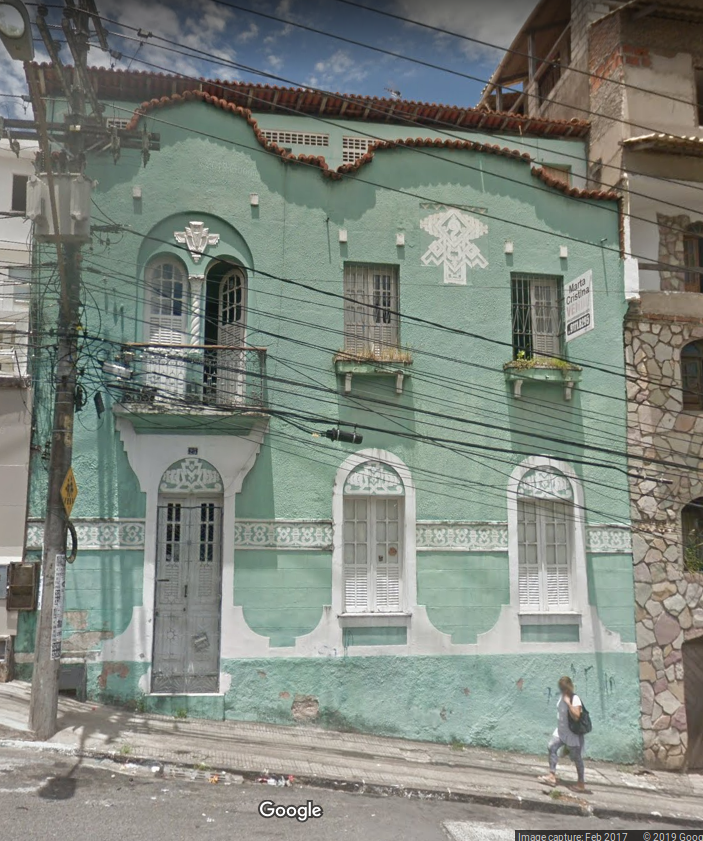
\includegraphics[width=1\textwidth]{8-anexos/plantas/01-1distrito/12-gales/ladeiradosgales-edmundoguimaraes-casa2017.jpg}{\footnotesize \par \textbf{Fonte:} Google Maps. }
\label{fig:edmundoguimaraes2017}
\end{figure}
}